\documentclass[10pt]{beamer}

\usepackage[utf8]{inputenc}
\usepackage[spanish]{babel}
\usepackage{graphicx}

\mode<presentation>
\usetheme{Madrid}
%\usecolortheme[RGB={111,73,135}]{structure}
\usecolortheme[RGB={128,0,0}]{structure}
%\usecolortheme[RGB={0,96,0}]{structure}
%\usecolortheme[RGB={200,0,200}]{structure}
%\usecolortheme[RGB={0,128,0}]{structure}
%\usecolortheme[RGB={0,0,128}]{structure}
\usefonttheme{serif}
\useinnertheme{rectangles}
\useoutertheme{split}
\setbeamercovered{transparent}


% Definiciones para usar luego
\newtheorem{ejemplo}{Ejemplo}
\newtheorem{definicion}{Definición}

\title{Sistemas de Ficheros}
\author{Jesús Espino García}
\date{3 de Marzo de 2010}
\subject{Sistemas de Ficheros}

\institute[GUL UC3M]{
  Grupo de Usuarios de Linux\\
  Universidad Carlos III de Madrid.\\
  \ \\
  
\includegraphics[height=1.5cm]{imgs/gul}}

\setcounter{tocdepth}{2}

\AtBeginSubsection[]
{
  \begin{frame}<beamer>{Indice}
    \tableofcontents[sectionstyle=show/shaded,subsectionstyle=show/shaded/hide]
  \end{frame}
}

\begin{document}

  \frame{\maketitle}
  
  \section*{Introducción}
\subsection*{Conceptos Básicos}
\begin{frame}{Términos}
  \begin{itemize}
    \item Sistema de ficheros: Conjunto de algoritmos y datos que nos permiten almacenar nuestros datos y acceder a ellos en un dispositivo físico.
    \item Sector: Unidad de almacenamiento en disco.
    \item Bloque/Sector: Conjunto de sectores contiguos que conforman la unidad de almacenamiento más pequeña de la partición.
    \item Inodo: Estructura de datos que almacena un objeto del sistema de ficheros.
    \item Sector de Arranque: Zona de la partición reservada para el arranque del sistema operativo.
    \item Superblock: Bloque de datos que contiene información referente a toda la partición.
    \item Trashing: Ineficiencia producida en un sistema de ficheros debido al excesivo movimiento de los cabezales del disco duro.
    \item Extent: Conjunto de bloques contiguos y relacionados.
  \end{itemize}
\end{frame}

\begin{frame}{Journaling}
  \begin{itemize}
    \item Sistema de seguridad de los sistemas de ficheros para preservar la consistencia.
    \item Guarda información de las operaciones para poder dar marcha atrás en caso de ser necesario.
    \item El proceso de journaling es sencillo:
    \begin{itemize}
      \item Se bloquean las estructuras afectadas.
      \item Se crea el journal.
      \item Se va apuntando y realizando las operaciones en el journal.
      \item Al terminar, si todo ha ido bien, se elimina el journal.
    \end{itemize}
    \item En los sistemas de fichero se suelen usar únicamente para los metadatos.
  \end{itemize}
\end{frame}

\begin{frame}{ACLs}
  \begin{itemize}
    \item Listas de control de acceso.
    \item Permiten un control de acceso muy granular.
    \item Se define quién accede a qué y con qué permisos.
  \end{itemize}
\end{frame}

\begin{frame}{Arboles B+}
  \begin{itemize}
    \item Árbol donde sólo los nodos hoja tiene información.
    \item Los nodos hojas están enlazados entre si (para acceso secuencial).
    \item Usado para acceso y borrado de forma eficiente.
  \end{itemize}
\end{frame}

\subsection*{Tipos de Sistemas de Ficheros}
\begin{frame}{Tipos de Sistemas de Ficheros}
  \begin{itemize}
    \item Sistemas de disco: Diseñados para almacenar ficheros en un dispositivo de almacenamiento de datos (Ej: disco duro, cdrom, dvd, discos de memoria, etc).
    \item Sistemas de ficheros de bases de datos: Están basados en metadatos, de este modo las búsquedas se realizan por consultas a dicha base de datos (Ej: Gnome VFS, BFS, WinFS,etc).
    \item Sistemas de ficheros transaccionales: Sistemas de ficheros que soportan transacciones.
    \item Sistemas de ficheros de propósito especifico: Sus contenidos son generados directamente por software (Ej: /proc, /sys, etc).
  \end{itemize}
\end{frame}

  \section{Ext 2/3/4}
\subsection{Introducción}
\begin{frame}{Introducción}
  \begin{itemize}
    \item Surgio como sustituo para el sistema Minix en Linux.
    \item En abril del 92 fue liberado la version 1 usando ya la API VFS de Linux.
    \item Soluciono gran parte de los problemas que planteaba Minix (Principalmente tamaño maximo y numero de caracteres).
    \item En el 93 aparece su version 2 incorporando ideas de Berkeley Fast File System y pensado para escabilidad.
  \end{itemize}
\end{frame}

\subsection{Caracteristicas}
\begin{frame}{Caracteristicas ext2}
  \begin{itemize}
    \item Permisos POSIX
    \item ACLs
    \item Tamaño maximo: 8TB
    \item Tamaño maximo de fichero: 2TB
    \item Maximo de caracteres de nombre de fichero: 255B
    \item Maximo numero de ficheros: NA
  \end{itemize}
\end{frame}

\begin{frame}{Caracteristicas ext3}
  \begin{itemize}
    \item Journaling
    \item ACLs
    \item Extents (Actualización)
    \item Tamaño maximo: 8TB
    \item Tamaño maximo de fichero: 2TB
    \item Maximo de caracteres de nombre de fichero: 255B
    \item Maximo numero de ficheros: NA
  \end{itemize}
\end{frame}

\begin{frame}{Caracteristicas ext4}
  \begin{itemize}
    \item Journaling
    \item ACLs
    \item Extents
    \item Tamaño maximo: 1EB
    \item Tamaño maximo de fichero: 16TB
    \item Maximo de caracteres de nombre de fichero: 255B
    \item Maximo numero de ficheros: 4.000.000.000
  \end{itemize}
\end{frame}

\subsection{Estructura}
\begin{frame}{Estructura}
  \begin{itemize}
    \item Al principio de la particion nos encontramos el sector de arranque.
    \item El resto del espacio (practicamente todo) se divide en grupos de bloques.
    \item Cada grupo de bloques contiene:
    \begin{itemize}
      \item Si es el primero un superbloque, si no, puede o no contener un backup de el superbloque.
      \item Un descriptor de grupo, que contiene informacion sobre el grupo de bloques.
      \item Un mapa de bits de bloques, que contiene informacion sobre los bloques libres.
      \item Un mapa de bits de inodos, que contiene infomacion sobre los inodos libres.
      \item Bloque de datos, que contiene los datos de los ficheros.
    \end{itemize}
  \end{itemize}
\end{frame}

\begin{frame}{Estructura}
  \begin{center}
    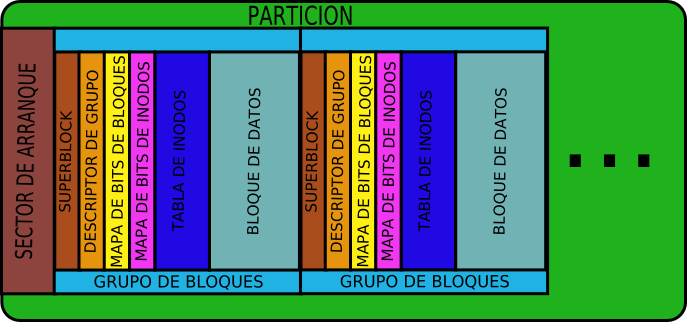
\includegraphics[height=5.5cm]{imgs/ext_struct.png}
  \end{center}
\end{frame}

\begin{frame}{Ficheros}
  \begin{itemize}
    \item La informacion de los ficheros se almacena en los inodos. Un fichero puede ser un directorio, un fichero regular, un socket, etc...
    \item En el inodo no se almacenan datos, solo punteros a los bloques de datos o extents.
    \item Los punteros a los bloques de datos pueden ser:
    \begin{itemize}
      \item Directos: Apuntan directamente a un bloque de datos
      \item Indirectos: Apuntan a un bloque de punteros directos.
      \item Doblemente indirectos: Apuntan a un bloque de punteros indirectos.
      \item Triplemente indirectos: Apuntan a un bloque de puntersos doblemente indirectos.
    \end{itemize}
    \item Los extents se representan dentro de un arbol B+:
    \begin{itemize}
      \item Cualquier nodo intermedio contiene una serie de indices que apuntan a nodos hijos.
      \item Los nodos hoja continen estructuras extent que apuntan a un conjunto de bloques.
    \end{itemize}
    \item Los datos almacenados en los directorios son el nombre del fichero y el inodo que lo contiene.
  \end{itemize}
\end{frame}

\begin{frame}{Ficheros}
  \begin{center}
    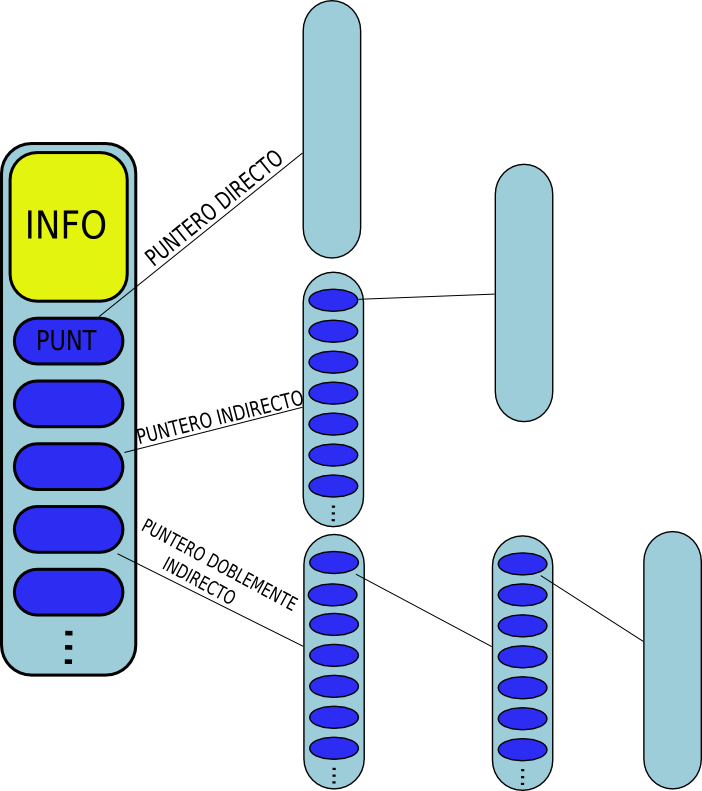
\includegraphics[height=6cm]{imgs/ext_files.png}
  \end{center}
\end{frame}

  \section{FAT}
\subsection{Introducción}
\begin{frame}{Introducción}
  \begin{itemize}
    \item Creado por Bill Gates y Marc McDonald.
    \item Se creó en 1977.
    \item Su primera versión fue FAT12 (con direcciones de 12 bits).
    \item Posteriormente apareció FAT16.
    \item Finalmente se llegó a FAT32 (el actual) (28 bits).
  \end{itemize}
\end{frame}

\subsection{Características}
\begin{frame}{Características}
  \begin{itemize}
    \item Tamaño máximo: 32GB
    \item Tamaño máximo de fichero: 4GB
    \item Máximo de caracteres de nombre de fichero: 255B
    \item Máximo número de ficheros: 4.177.920
  \end{itemize}
\end{frame}

\subsection{Estructura}
\begin{frame}{Estructura}
  \begin{itemize}
    \item Al principio de la partición nos encontramos el sector de arranque.
    \item Justo después se encuentra la FAT
    \item Normalmente (pero no necesariamente) encontramos después el directorio raíz.
    \item Después nos encontramos el área de datos, donde se almacenan todos los ficheros.
  \end{itemize}
\end{frame}

\begin{frame}{Estructura}
  \begin{center}
    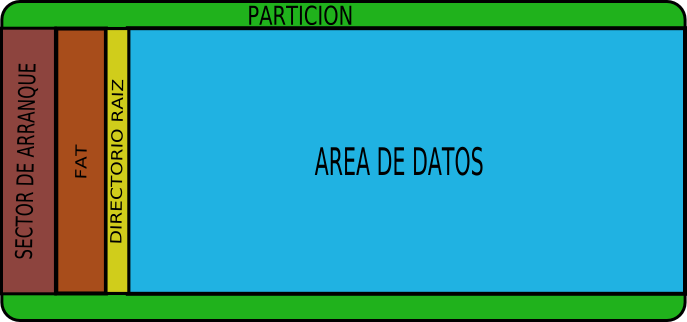
\includegraphics[height=5.5cm]{imgs/fat_struct.png}
  \end{center}
\end{frame}

\begin{frame}{Ficheros}
  \begin{itemize}
    \item Los ficheros única y exclusivamente contienen datos y están almacenados en el sector de datos de la partición.
    \item Las entradas de directorios almacenan el nombre, el número de cluster y los atributos de cada uno de los ficheros que contiene.
    \item Los ficheros vacíos no contienen ocupan bloques de datos ni entradas en la fat.
    \item Si un cluster no es el ultimo del fichero, contiene el número de cluster siguiente, si lo es, contiene una marca.
    \item Los directorios siempre contiene como mínimo los subdirectorios "." y "..", excepto el directorio raíz.
  \end{itemize}
\end{frame}

\begin{frame}{Ficheros}
  \begin{center}
    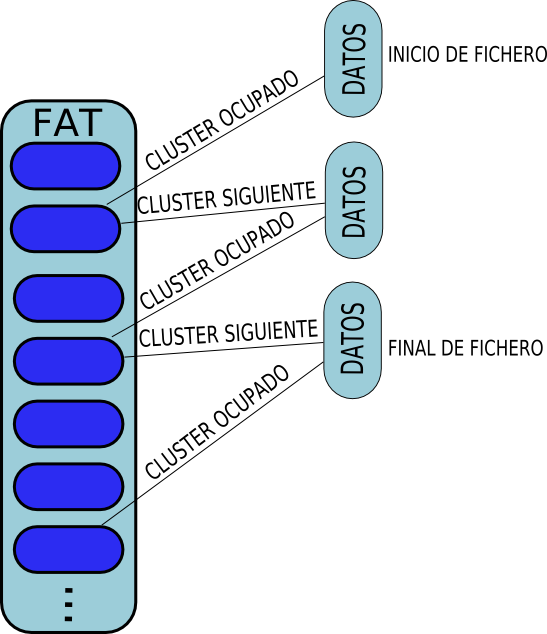
\includegraphics[height=6cm]{imgs/fat_files.png}
  \end{center}
\end{frame}

  \section{NTFS}
\subsection{Introducción}
\begin{frame}{Introducción}
  \begin{itemize}
    \item Reemplazo de Microsoft para los sistemas FAT.
    \item Mejoras importantes como soporte de metadatos y uso de estructuras de datos avanzadas.
    \item Debido a que sus especificaciones son secretas no tiene buen soporte en sistemas no Microsoft.
  \end{itemize}
\end{frame}

\subsection{Características}
\begin{frame}{Características}
  \begin{itemize}
    \item Journaling (Solo para la parte de metadatos)
    \item ACLs
    \item Cifrado
    \item Compresion
    \item Tamaño máximo: 16TB
    \item Tamaño máximo de fichero: 16TB
    \item Máximo de caracteres de nombre de fichero: 256B
    \item Máximo número de ficheros: 4.294.967.295
  \end{itemize}
\end{frame}

\subsection{Estructura}
\begin{frame}{Estructura}
  \begin{itemize}
    \item Al principio de la partición nos encontramos el sector de arranque.
    \item Justo después se encuentra la MFT (Master File Table).
    \item Cada entrada del MFT es un fichero del sistema de ficheros.
    \item Las primeras 16 entradas de la MFT son ficheros de metadatos.
    \item Después tenemos el área de datos.
    \item En medio de la partición, aproximadamente, nos encontramos una copia de la MFT.
    \item Al final de la partición nos encontramos un backup del sector de arranque.
  \end{itemize}
\end{frame}

\begin{frame}{Estructura}
  \begin{center}
    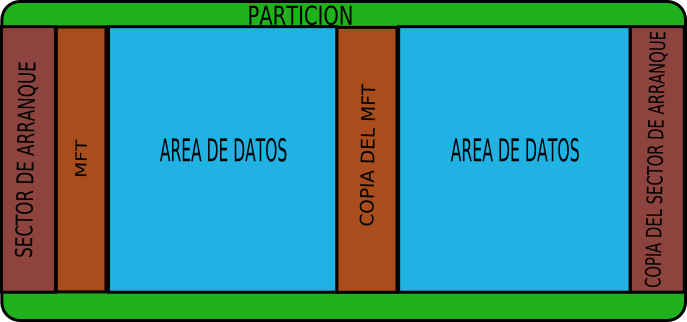
\includegraphics[height=5.5cm]{imgs/ntfs_struct.png}
  \end{center}
\end{frame}

\begin{frame}{Ficheros}
  \begin{itemize}
    \item Los ficheros contienen información sobre el fichero, atributos y características.
    \item Si el fichero es pequeño lo incluye directamente en el MFT.
    \item Si el fichero es grande va almacenando los datos en ``extents`` (grupos de clusters fuera del MFT).
    \item Si el fichero fuera tan grande que no cupieran más direcciones de ``extents``, externalizaría las direcciones.
    \item De este modo seguiría creciendo hasta que no se necesite más espacio.
    \item Los directorios contiene los ficheros ordenados a modo de arbol B.
  \end{itemize}
\end{frame}

\begin{frame}{Ficheros}
  \begin{center}
    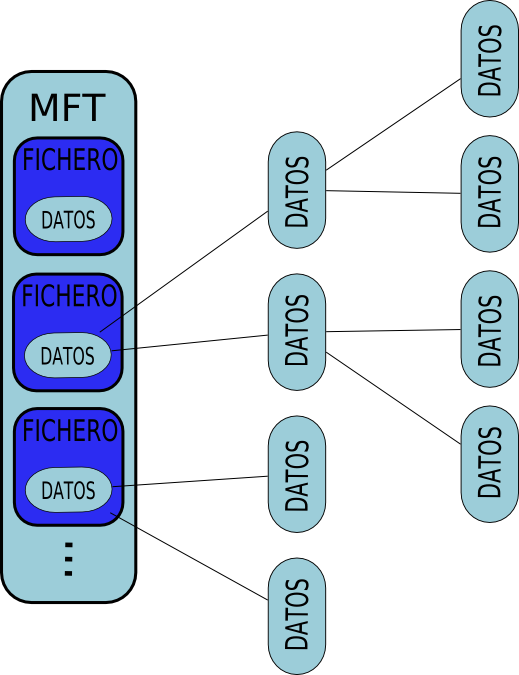
\includegraphics[height=6cm]{imgs/ntfs_files.png}
  \end{center}
\end{frame}

  \section{ReiserFS}
\subsection{Introducción}
\begin{frame}{Introducción}
  \begin{itemize}
    \item Sistema de propósito general.
    \item Muy bueno en tratamiento de ficheros pequeños.
    \item Primero sistema de ficheros con Journaling incluido en el kernel de Linux.
    \item Es el sistema de ficheros por defecto en varias distribuciones.
    \item Actualmente Namesys ha dejado el desarrollo de ReiserFS para centrarse en su sucesor Reiser4.
  \end{itemize}
\end{frame}

\subsection{Características}
\begin{frame}{Características}
  \begin{itemize}
    \item Journaling
    \item ACLs
    \item Permisos POSIX
    \item Tamaño máximo: 16TB
    \item Tamaño máximo de fichero: 16TB
    \item Máximo de caracteres de nombre de fichero: 256B
    \item Máximo número de ficheros: 4.294.967.293
  \end{itemize}
\end{frame}

\subsection{Estructura}
\begin{frame}{Estructura}
  \begin{itemize}
    \item Al principio de la partición nos encontramos el sector de arranque.
    \item Justo después se encuentra el superblock.
    \item Para el resto de la partición se van alternando mapas de bits de bloques y bloques de datos.
    \item Cada mapa de bits de bloques se refiere al bloque de datos que queda después de el y nos da información sobre los bloques libres  y ocupados.
    \item Cada bloque de datos contiene los datos e inodos.
  \end{itemize}
\end{frame}

\begin{frame}{Estructura}
  \begin{center}
    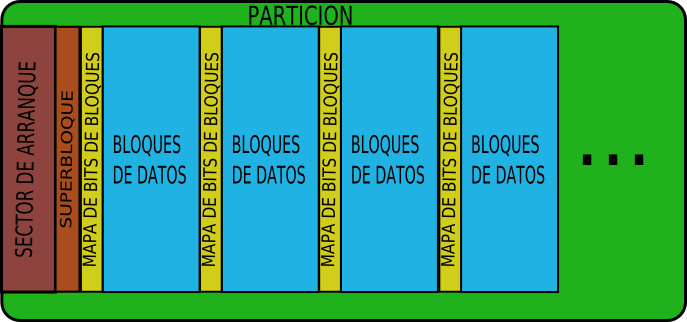
\includegraphics[height=5.5cm]{imgs/reiserfs_struct.png}
  \end{center}
\end{frame}

\begin{frame}{Ficheros}
  \begin{itemize}
    \item Existen 4 tipos de objetos: stat, directorios, directos e indirectos.
    \item Todos los ficheros en reiser tienen asociado un objeto stat, el cual almacena información de permisos.
    \item Los directorios a su vez tienen asociados uno o más objetos del tipo directorio, tantos como hagan falta para almacenar todas las entradas del directorio.
    \item Los ficheros regulares, si son pequeños se asocian a un objeto directo que almacena los datos, si son grandes se asocia a uno o varios objetos indirectos que contienen punteros a bloques de datos.
  \end{itemize}
\end{frame}

\begin{frame}{Ficheros}
  \begin{center}
    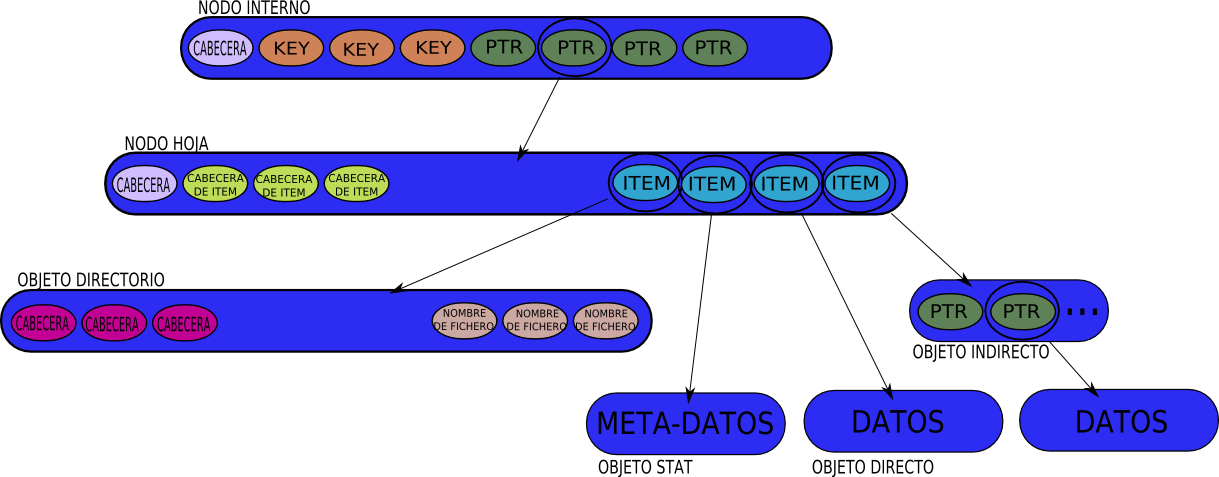
\includegraphics[height=4.5cm]{imgs/reiserfs_files.png}
  \end{center}
\end{frame}

  \section{XFS}
\subsection{Introducción}
\begin{frame}{Introducción}
  \begin{itemize}
    \item Creado por Silicon Graphics para IRIX.
    \item Liberado bajo licencia GPL en Mayo del 2000.
    \item Actualmente incluido en el kernel de Linux
    \item Opción en muchas distribuciones.
  \end{itemize}
\end{frame}

\subsection{Características}
\begin{frame}{Características}
  \begin{itemize}
    \item Journaling (Solo para los metadatos)
    \item ACLs
    \item Permisos POSIX
    \item Tamaño máximo: 9EB
    \item Tamaño máximo de fichero: 9EB
    \item Máximo de caracteres de nombre de fichero: 255B
    \item Máximo número de ficheros: NA
  \end{itemize}
\end{frame}

\subsection{Estructura}
\begin{frame}{Estructura}
  \begin{itemize}
    \item En XFS no existe el espacio para el sector de arranque.
    \item El espacio se divide completamente en \"Grupos de Asignación\"
    \item Cada grupo de asignación esta compuesto por:
    \begin{itemize}
      \item El superbloque (Si no es el primer grupo, solo es una copia).
      \item Un espacio para información de asignación de bloques e inodos del grupo (almacenada en arboles B+).
      \item Y un bloque de datos donde se almacenan los inodos y bloques de datos.
    \end{itemize}
  \end{itemize}
\end{frame}

\begin{frame}{Estructura}
  \begin{center}
    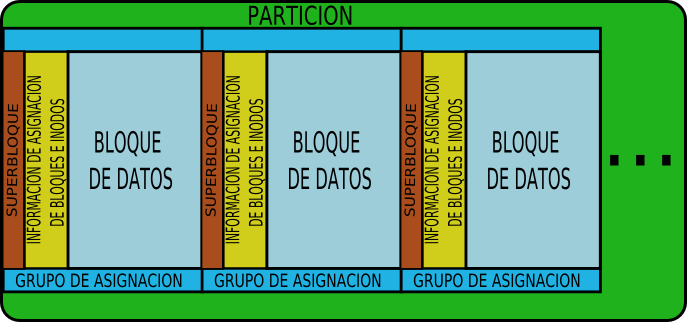
\includegraphics[height=5.5cm]{imgs/xfs_struct.png}
  \end{center}
\end{frame}

\begin{frame}{Ficheros}
  \begin{itemize}
    \item Los inodos contienen un núcleo con la información básica.
    \item Para especificar los bloques de datos usa \"extents\", es decir, dirección inicial y tamaño total.
    \item Los inodos pueden tener almacenar los datos del fichero de tres maneras:
    \begin{itemize}
      \item NULO: No hay ningún dato, por lo tanto no hay extents.
      \item EXTENTS: Un mapa de extents de bloques de datos.
      \item B+ EXTENTS: Un árbol B+ de extents en el que los nodos hoja son bloques de datos.
    \end{itemize}
  \end{itemize}
\end{frame}

\begin{frame}{Ficheros}
  \begin{center}
    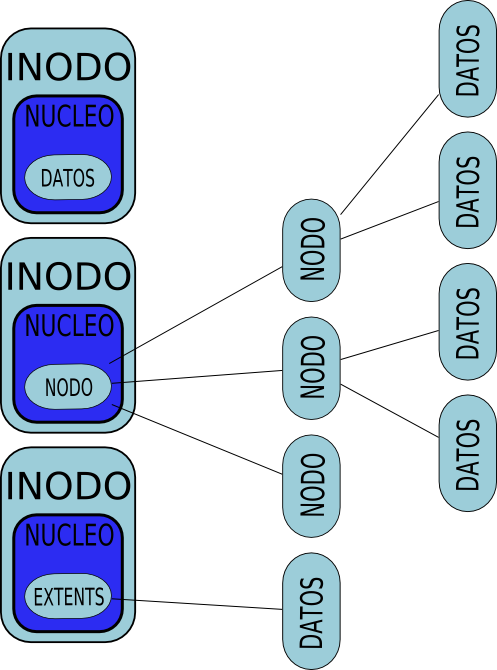
\includegraphics[height=6cm]{imgs/xfs_files.png}
  \end{center}
\end{frame}

  \include{fs_jfs}
  \include{fs_btrfs}

\end{document}
